\section{Estrutura}

O interpretador é simples e consiste somente de 
três grandes fases: \textit{lexer}, \textit{parser}
e \textit{evaluator}, representados na figura
\ref{fig:pipeline}.
\index{pipeline}
\index{interpretador}
\index{lexer} \index{parser} \index{evaluator}

\begin{figure}
    \centering
    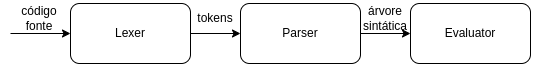
\includegraphics[width=0.75\linewidth]{pipeline.png}
    \caption{Pipeline do interpretador}
    \label{fig:pipeline}
\end{figure}

Por vezes, na literatura, lexers são chamados de
\textit{scanners}, \textit{escaneadores},
\textit{tokenizer}, \textit{analisadores léxicos}, etc;
e parsers são chamados de \textit{analisadores sintáticos};
\index{tokenizer} \index{scanner} \index{analisador léxico}
\index{analisador sintático}

Com o objetivo de interpretar o código, não é vantajoso
olharmos para o código-fonte diretamente como caracteres.
Ao invés disso, construímos uma sequência de abstrações,
uma em cima da outra, até que o código esteja em um formato
fácil de ser interpretado.

\index{lexemas} \index{tokens}
A primeira abstração são os \textit{lexemas} (também chamados
de \textit{tokens}), produzidos pelo
\textit{lexer}. Os lexemas são estruturas simples que
classificam pedaços do código fonte. São implementados
pelo objeto:

\begin{lstlisting}
class Lexeme:
    def __init__(self, string, kind, range):
        self.text = string
        self.kind = kind
        self.range = range
\end{lstlisting}

\noindent Veja que ele contém apenas um pedaço do código fonte
(\verb|text|), uma classificação (\verb|kind|) e
a posição desse lexema no código fonte (\verb|range|).

\index{fatorial}
Por exemplo, considere a função \verb|fact| declarada
a seguir:

\begin{lstlisting}
def fact(n):
    if n <= 0:
        return 1
    return n * fact(n-1)
\end{lstlisting}

A primeira linha é transformada na seguinte sequência de
lexemas:

\begin{lstlisting}
('def', DEF)
('fact', ID)
('(', LEFT_PAREN)
('n', ID)
(')', RIGHT_PAREN)
(':', COLON)
\end{lstlisting}

\noindent Representados como \verb|(<text>, <kind>)|.
É possível gerar os lexemas de um arquivo com o
comando: \verb|spy lex <file>|.

\index{lexemas}
Os lexemas já facilitam muito o processamento do texto,
mas para interpretação, precisamos capturar a estrutura
do código fonte: onde começam e terminam
as declarações de função, onde começam e terminam
os blocos de código, as expressões, etc. Para esse fim, 
utilizamos as \textit{árvores sintáticas}.
\index{árvores sintáticas}

\begin{lstlisting}
# value precisa ser um Lexeme
class Node:
    def __init__(self, value, kind):
        self.value = value
        self.kind = kind
        self.leaves = []
        self.range = None
\end{lstlisting}

As árvores sintáticas são árvores n-árias que abstraem a
estrutura do código fonte. Podemos representar a árvore
da função \verb|fact| usando indentação da seguinte forma:

\begin{lstlisting}
FUNC
  TERMINAL ('fact', ID)
  ARG_LIST
    TERMINAL ('n', ID)
  BLOCK
    IF
      ...
    RETURN
      ...
\end{lstlisting}

É possível gerar a árvore sintática de um arquivo
com o seguinte comando: \verb|spy parse <file>|.